\section{Sensores}
\label{sec:sensors}
Para navegar de manera robusta a través de entornos desconocidos y no estructurados, los robots deben poder percibir y modelar su entorno. Es por esto que lo que se busca es construir mapas precisos y ubicarse en los mismos utilizando solo sensores a bordo. Dentro de los mismos pueden diferenciarse dos grandes grupos
\begin{itemize}
    \item En primer lugar, los sensores necesarios para obtener información de los \textit{alrededores} del robot, como pueden ser el LIDAR y la cámara. Estos se los denominan \textit{sensores exteroceptivos}. Un sistema SLAM mínimo requiere al menos de uno de ellos para poder realizar dicha tarea.
    \item Opcionalmente, aquellos sensores que miden el movimiento propio del robot, como pueden ser los acelerómetros y encoders, los que se denominan \textit{sensores propioceptivos}.
\end{itemize}

\subsection{LiDAR}
Light Detection And Ranging, conocido como LiDAR, es una tecnología que tiene su origen en la fusión de la tecnología láser junto con la tecnología RADAR (Radio Detection And Ranging), lo cual ha permitido mejorar en gran medida la precisión de los sistemas de detección, dando lugar a nuevas aplicaciones. Los sensores LIDAR son actualmente una de las opciones más confiables para SLAM robótico tanto en ambientes interiores como exteriores. Los mismos exhibien fuentes y tipos de ruido similares que pueden modelarse libremente como Gaussianos \textbf{[133]}.

Muchos investigadores tienen sensores LiDAR de exploración servo-montados en configuraciones de cabeceo \textbf{[116, 117]} o de barrido \textbf{[118]} (Figura \ref{fig:lidars}.a) para producir exploraciones tanto planares como 3D, aunque para este último caso el mismo entrega escaneos cada 1Hz o menos. Este campo de visión, sobre todo el 3D, tiene el costo de una mayor complejidad (sincronización servo temporal) y una menor cobertura en direcciones críticas.
\textbf{[pfingsthron2012] [newman2006] [bosse2009]}

Con el fin de aumentar la frecuencia de recolección de datos, existen sensores que integran múltiples LiDAR en una sola unidad de escaneo (Figura \ref{fig:lidars}.b), de modo que se pueden obtener escaneados en 3D completos a altas velocidades.

\begin{figure}[!b]
    \centering
    \subfloat[Scanse Sweep]{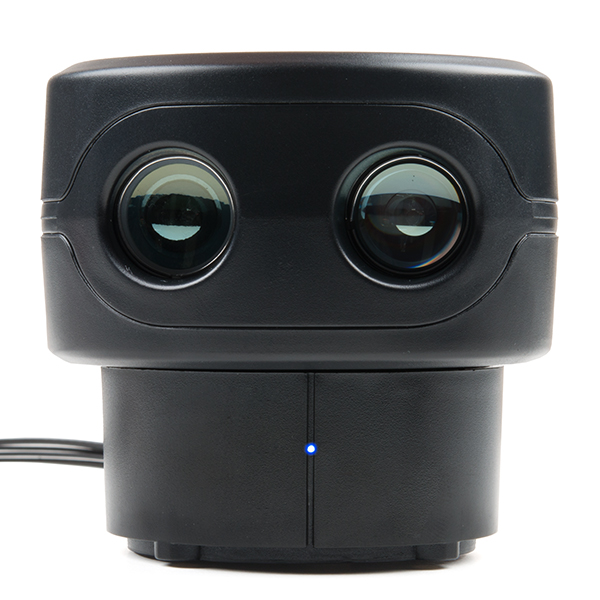
\includegraphics[width=.35\textwidth]{Img/scanse-sweep}}
    \qquad
    \subfloat[Velodyne VLP-16]{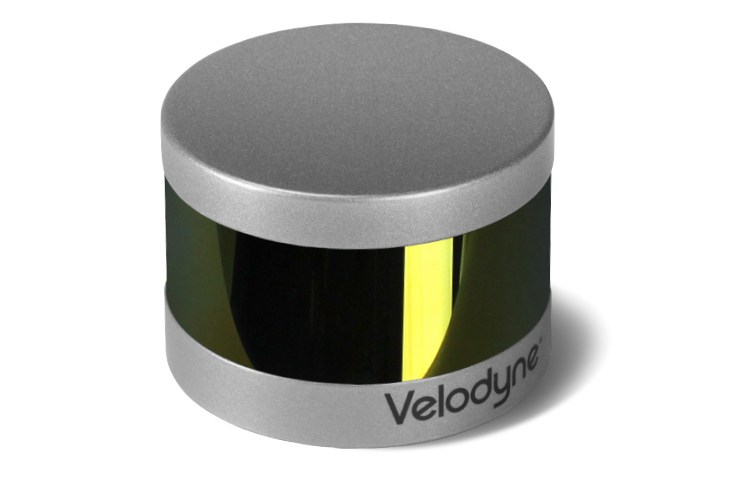
\includegraphics[width=.5\textwidth]{Img/vlp-16}}
    \caption{Algunos LIDAR comerciales}
    \label{fig:lidars}
\end{figure}

\subsubsection{Principio de funcionamiento}
El  fundamento de los dispositivos basados en la tecnología LIDAR es el cálculo del tiempo de vuelo (\textit{ToF - Time  Of Flight}) de los pulsos láser, de manera que, conociendo la velocidad del mismo, las características angulares con las que fue emitido, y la diferencia de tiempos entre el rayo emitido y el reflejado, se puede determinar de manera sencilla la distancia a la que se encuentra el obstáculo/objeto con el que el rayo impactó. Esto permite, con gran exactitud, conocer las coordenadas de la posición de objetos o superficies con respecto del sistema de coordenadas del propio dispositivo.

A medida que cada pulso láser diverge, traza un volumen que es aproximadamente cónico. Si alguna parte de este volumen cónico se cruza con un objeto, parte de la luz reflejada puede regresar a través de la lente del LIDAR. Una vez que la parte frontal del receptor del LIDAR ha recogido suficiente luz (es decir, con un umbral) registra el retorno y calcula la distancia. Esta señal de entrada introduce efectos de acortamiento y alargamiento de rango.

\subsubsection{Fuentes de ruido}
Algunas de las fuentes de ruido que afectan a la medición del LIDAR son
\begin{itemize}
    \item \textit{Ángulo de incidencia:} Si un pulso LIDAR golpea una superficie perpendicularmente, todo el frente de la onda láser se refleja al mismo tiempo. Sin embargo, a medida que aumenta el ángulo de incidencia, parte del frente de onda se refleja antes y la señal recibida activará el umbral, tarde o temprano, dependiendo del diseño del detector frontal. A medida que el ángulo de incidencia se acerca a los 90 grados, una configuración común para el lidar montado horizontalmente, los pulsos lidar viajan casi paralelos al suelo. Estos retornos de ''pastoreo en el suelo'' son extremadamente sensibles al tono del robot, las variaciones en la superficie y otros ruidos. En esta configuración, incluso un robot sin movimiento puede producir mediciones lidar con medidores de ruido de rango. Estos retornos de pastoreo pueden presentar un desafío para SLAM con un lidar montado horizontalmente.
    \item \textit{Efectos de contorno:} están estrechamente relacionados con los retornos de pastoreo, los retornos espurios pueden ocurrir en el límite de los objetos, donde el frente de onda elíptica puede intersecar parte de uno o más objetos a medida que viaja. La medición del rango resultante a menudo se promedia y se crea una medición espuria "colgando" en el espacio vacío entre los objetos. La figura 2.4 demuestra este efecto.
    \item \textit{Propiedades de la superficie del objeto:} causa que la cantidad de luz láser reflejada varíe mucho. Un objeto altamente especular, como un espejo o agua quieta, reflejará la mayor parte de la luz láser y, a menudo, devolverá las mediciones a objetos más distantes (en el rumbo incorrecto). Cuanto más difusamente un objeto refleje la luz, mejor se puede medir en un rango más amplio de ángulos y distancias. Los objetos que absorben la luz infrarroja (que generalmente se ve negra para los humanos) a menudo no pueden reflejar suficiente luz, lo que limita los rangos de medición. Además, en algunos sensores lidar, los objetos blancos pueden aparecer un poco más cerca que los objetos negros, ya que el umbral del receptor se activa un poco antes [133].
    \item \textit{Luz ambiental:} La mayoría de los sensores comerciales LIDAR utilizan filtros de muesca infrarrojos para aumentar la relación señal a ruido. Si bien esto les permite funcionar al aire libre, la luz ambiental intensa, como la luz solar directa, disminuirá su alcance. Cuando la luz reflejada de un pulso lidar no es lo suficientemente fuerte como para activar una medición, un modelo de sensor típico supone que hay espacio libre hasta una fracción del rango máximo del sensor. Esta suposición de espacio libre debe variar según los niveles de luz ambiental, sin embargo, sin sensores adicionales, no es posible determinar cuándo la medición de lidar faltante se debe al espacio libre real o a la luz ambiental excesiva.
    \item \textit{Sincronización temporal:} cuando se monta en un robot en movimiento, el origen de un lidar se moverá a medida que el sensor giratorio complete cada escaneo. Moviéndose a $1m/s$, por ejemplo, un lidar de 40 Hz producirá hasta 25 mm de sesgo si no se compensa. La compensación se puede realizar utilizando un modelo de movimiento continuo, como [134], sin embargo, esto requiere una sincronización rigurosa y una marca de tiempo de los datos del sensor. La figura 2.4 muestra una nube de puntos tridimensional coloreada generada a partir de un lidar montado en un servomotor de movimiento rápido, con una cámara de obturación global y sincronización de microsegundos.
\end{itemize}

\subsubsection{Calibración}
La calibración de los LIDAR puede realizarse mediante el uso de planos conocidos \textbf{(Habib, 2010)}, aunque también mediante el uso de sensores adicionales, siendo el más común la cámara, ya que de la misma pueden asociarse los puntos relacionados entre ambos sensores \textbf{(An, 2020)}, e incluso con el agregado de sensores adicionales \textbf{(Domhof, 2019)}. Sin embargo, la ubicación en la que se encuentra cada sensor exactamente puede ser una tarea complicada, pero existen en la literatura diferentes enfoques para realizarlo \textbf{(Kim, 2020)}.

\subsection{Cámara}
Las cámaras en su versión más simple tienen la característica de ser más económicas y sencillas de montar respecto al resto de los sensores utilizados para el SLAM (tal como el LiDAR), además de no emitir señales al entorno para obtener las características del mismo. A la hora de realizar el SLAM. el modelo de sensado de las cámaras consiste básicamente en un mapeo entre el entorno tridimencional y el plano de la imagen bidimensional. Dependiendo del tipo de cámara (monocular, estéreo, omnidireccional, RGB-D, entre otras), es posible utilizar diferentes modelos matemáticos que permitan relacionar puntos del mundo con su respectiva representación en la imagen.

Para las cámaras monoculares, la línea de base entre las imágenes debe estimarse a partir de la odometría, lo que da lugar al problema de SLAM monocular bien estudiado [124, 125]. Otra forma de realizarlo es mediante la percepción de alto nivel, donde se pueden utilizar señales como el tamaño relativo de un objeto para estimar la escala de la imagen y, por lo tanto, la profundidad [126].

En cambio, para las cámaras RGB-D (\textit{D: Depth} - Profundidad) (Figura \ref{fig:camaras}.b), uno de los métodos presentados en la literatura para la realización del SLAM a partir de las mismas [ENDERS2012] consiste en primero extraer características visuales de las imágenes de color entrantes. Luego, se comparan estas características con las características de imágenes anteriores. Al evaluar las imágenes de profundidad en las ubicaciones de estos puntos de características, se obtienen un conjunto de correspondencias 3D puntuales entre dos cuadros cualquiera. Basándose en estas correspondencias, se estima la transformación relativa entre los marcos utilizando RANSAC \textbf{[Trivedi,2013]}.

Por otro lado, las técnicas de visión estéreo utilizan dos cámaras con una separación entre las mismas fija y conocida (Figura \ref{fig:camaras}.a). Las correspondencias de características de la imagen se identifican entre las imágenes mediante la geometría epipolar[REF DE CASTRO] [111], y los rangos se calculan cuando se han medido las disparidades de imagen. Los enfoques pasivos sufren desde muchos modos de falla, desde agujeros de profundidad en áreas de imagen sin características visuales, hasta escenas que crean ambigüedades [123].

\begin{figure}
    \centering
    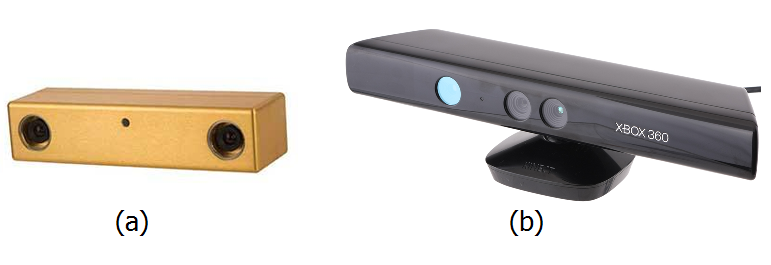
\includegraphics[width=.9\textwidth]{Img/bumblekinect}
    \caption{Cámaras: (a) Bumblebee 2, (b) Kinect}
    \label{fig:camaras}
\end{figure}

\subsubsection{Visión artificial}
La visión artificial consiste en la transformación de la información de una cámara quieta o de video en una decisión o una nueva representación. La decisión puede ser la detección de un patrón en la imagen, mientras que una nueva representación podría ser convertir una imagen en color a una en escala de grises.

\subsubsection{OpenCV}
OpenCV\footnote{http://opencv.org} es una librería open source multiplataforma que busca brindar una infraestructura de visión artificial fácil de usar y que pueda utilizarse para aplicaciones de tiempo real, por lo que hace hincapié en la optimización. Para ello, OpenCV cuenta con un set de más de 500 funciones\textbf{[Asano, 2012]} que abarcan muchas áreas en visión, tales como calibración de cámaras, visión estéreo y robótica.

\subsubsection{Cámara monocular}
La visión comienza con la detección de luz del ambiente. La geometría del viaje de los rayos de un objeto a través de la lente de la cámara, y el generador de imágenes es de particular importancia en visión artificial.


\paragraph{Modelo de la cámara}
Comenzando con el modelo ideal de la cámara, el cual es el agujero de alfiler (o \textit{pinhole}), aunque también llamada cámara estenopeica, como se observa en la Figura \ref{fig:pinholecamera} \textbf{REEMPLAZAR 1 POR $f$}. En la realidad, el plano de la imagen se encuentra detrás del pinhole, pero se muestra en el frente para evitar trabajar con imagenes giradas. Este es el denominado \textit{modelo de proyección frontal}. El eje $\undervec{\bm{s}}_3$ de $\undervec{\bm{\mathcal{F}}}_s$, llamado el \textit{eje 
óptico}, es ortogonal al plano de la imagen, y la distancia entre el pinhole, $S$, y el centro de plano de imagen, $C$,  se denomina la \textit{distancia focal}, $f$.
\begin{figure}
    \centering
    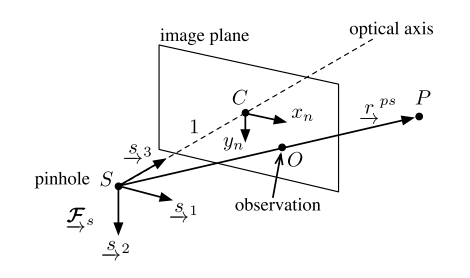
\includegraphics[width=\textwidth]{Img/PinholeCamera.png}
    \caption{Modelo de la cámara estenopeica}
    \label{fig:pinholecamera}
\end{figure}

Como los píxeles individuales de un generador de imágenes de bajo costo son rectangulares en lugar de ser cuadrados, las distancias focales para cada eje serán distintas. Por ejemplo, la distancia focal $f_x$ es el producto entre la distancia focal física del lente y el tamaño $s_x$ de los elementos individuales del generador de imágenes. De forma análoga, puede plantearse $f_y$.

Si las coordenadas de $P$ en $\undervec{\bm{\mathcal{F}}}_s$ son
\begin{equation}
    \bm{\rho} = \bm{r}_s^{ps} = 
    \begin{bmatrix}
        x \\
        y \\
        z
    \end{bmatrix}
\end{equation}
con el eje $\undervec{s}_3$ ortogonal al plano de la imagen, luego las coordenadas de $O$ en el plano de la imagen son
\begin{align}
    x_n = f_x \frac{x}{z} \\
    y_n = f_y \frac{y}{z}
\end{align}
denominadas las \textit{coordenadas de imagen normalizadas} \textbf{(ES POR EL $w=1$ O POR EL $f=1$ QUE ES NORMALIZADO?)}, y suelen representarse en la forma homogénea como
\begin{equation}
    \bm{p} =
    \begin{bmatrix}
        x_n \\
        y_n \\
        1
        \label{eq:homogeneousnormalizedimagecoordinates}
    \end{bmatrix}
\end{equation}

Sin embargo, el centro del generador de imágenes no se encuentra usualmente en el eje óptico. Para tener en cuenta este corrimiento, se introducen $c_x$ y $c_y$. En consecuencia, las coordenadas normalizadas de la imagen resultan
\begin{align}
    x_n = f_x \frac{x}{z} + c_x
    \label{eq:x_n}
    \\
    y_n = f_y \frac{y}{z} + c_y
    \label{eq:y_n}
\end{align}

Teniendo en cuenta estas últimas Expresiones, puede representarse al punto $P$ en la pantalla de proyección $O$ con coordenadas $(x_i,y_i)$ mediante una multiplicación matricial
\begin{equation}
    \bm{o}=
    \begin{bmatrix}
        x_i \\
        y_i \\
        w_i
    \end{bmatrix}
    =\bm{M}\bm{\rho}
\end{equation}
donde $\bm{M}$ es denominada la \textit{matriz intrínseca de la cámara}
\begin{equation}
    \bm{M} = 
    \begin{bmatrix}
        f_x & 0 & c_x \\
        0 & f_y & c_y \\
        0 & 0 & 1
    \end{bmatrix}
\end{equation}
Nótese que si se dividen a $\bm{o}$ por $w_i$, se llega entonces a la Expresión (\ref{eq:homogeneousnormalizedimagecoordinates}).

\paragraph{Distorsiones de la lente}
Las lentes, debido a problemas en la fabricación, en la realidad no son perfectas. Dichos problemas pueden clasificarse en
\begin{itemize}
    \item \textit{Distorsión radial}: surge como un resultado de la forma del lente, produciendo que los píxeles cerca de los bordes del generador de imágenes se distorsionen (conocido como el efecto ''ojo de pez''). En la práctica, esta distorsión es pequeña y puede caracterizarse por los primeros términos de la serie de Taylor alrededor del radio $r=0$. Para cámaras económicas suelen utilizarse los dos primeros términos, $k_1$ y $k_2$. Para cámaras muy distorsionadas, puede utilizarse un tercer término de distorsión radial, $k_3$. En concreto, la ubicación radial de un punto en el generador de imágenes se reescala mediante
        \begin{align}
            x_{corr} &= x_i (1 + k_1 r^2 + k_2 r^4 + k_3 r^6) \\
            y_{corr} & = y_i  (1 + k_1 r^2 + k_2 r^4 + k_3 r^6) 
        \end{align}
    \item \textit{Distorsión tangencial}: surge del proceso de ensamblaje de la cámara en su conjunto. Esta distorsión se caracteriza mínimamente con dos parámetros adicionales, $p_1$ y $p_2$, tales que
        \begin{align}
            x_{corr} &= x + \left[2p_1xy + p_x(r^2 + 2x^2)\right] \\
            y_{corr} &= y + \left[p_1(r^2+2y^2) + 2p_2xy\right]
        \end{align}
\end{itemize}

Por lo tanto, en total se cuentan con cinco coeficientes de distorsión. A partir de esto, se denomina al \textit{vector de distorsión} como
\begin{equation}
    \bm{D} = 
    \begin{bmatrix}
    k_1 & k_2 & p_1 & p_2 & k_3
    \end{bmatrix}
    \label{eq:distortionvector}
\end{equation}

\paragraph{Calibración}
La calibración de la cámara es importante para relacionar las mediciones de la misma con las mediciones del mundo real. Este proceso de calibración pretende calcular tanto la matriz intrínseca de la cámara, $\bm{M}$, como el vector de distorsión, $\bm{D}$. Para ello, la librería de OpenCV dispone de la función \texttt{cv::calibrateCamera()}, del que necesita de una estructura que tiene una cierta cantidad de puntos identificables e individuales, tal como puede ser un tablero de ajedrez (o \textit{chessboard}), como el observado en la Figura \ref{fig:chessboardcalibration}.a. Al observar esta estructura desde distintos ángulos, puede computarse la ubicación relativa y orientación de la cámara en el momento de cada imagen, así como los parámetros intrínsecos de la misma. Para proveer con vistas múltiples, suele rotarse y trasladarse el objeto, tomando las diferentes imágenes del mismo en cada uno de estas posiciones, como se observa en la Figura \ref{fig:chessboardcalibration}.b, mediante el uso de diversas funciones de OpenCV útiles para el caso\textbf{(Asano, 2012)}

\begin{figure}
    \centering
    \subfloat[Tablero de ajedrez de 8x6 utilizado para la calibración de cámaras]{{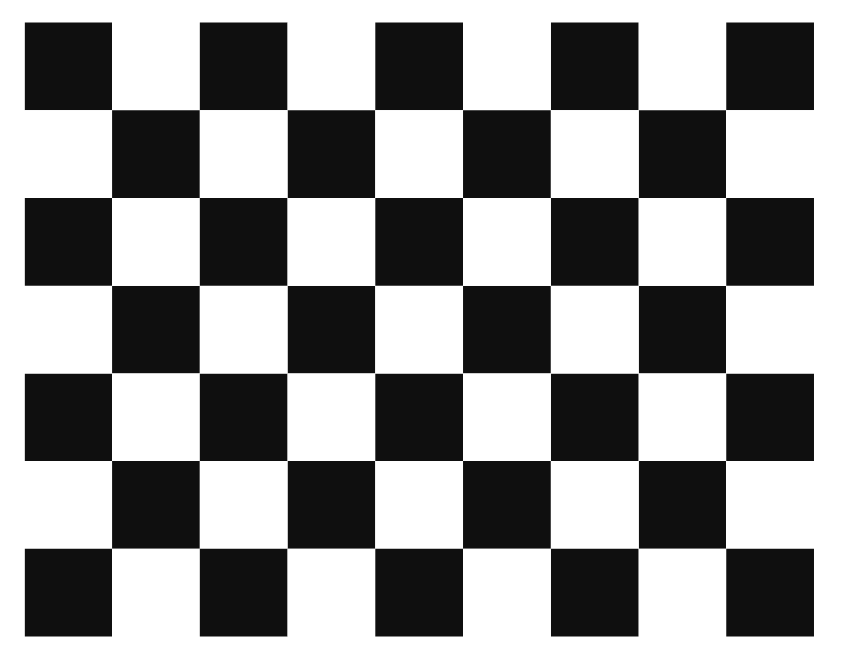
\includegraphics[width=0.45\textwidth]{Img/Chessboard.png}}}%
    \qquad
    \subfloat[Distintas posiciones del tablero de ajedrez]{{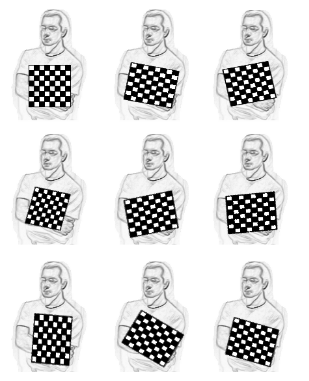
\includegraphics[width=0.35\textwidth]{Img/ChessboardVariousOrientations.png}}}%
    \caption{Tablero de ajedrez utilizado para la calibración de cámaras junto a sus distintas posiciones}
    \label{fig:chessboardcalibration}
\end{figure}

Como las dimensiones del objeto deben ser conocidas, para el caso del tablero suelen definirse el tamaño de los cuadrados y las intersecciones internas del mismo. Por ello, en la Figura \ref{fig:chessboardcalibration}.a el mismo es de 8x6.

\subparagraph{Calibración mediante ROS}
Para calibrar cámaras monoculares mediante ROS, se encuentra el paquete disponible \textit{camera calibration}\footnote{\url{http://wiki.ros.org/camera_calibration}}, el cual utiliza funciones de OpenCV para realizar dicha calibración, necesitando únicamente las dimensión del lado de los cuadrados del tablero utilizado (por ejemplo, 0.108 metros) y la dimensión del mismo (por ejemplo, 8x6). Una vez con dichos datos, se ejecuta el paquete, obteniéndose una pantalla como puede verse en la Figura \ref{fig:monocularcameracalibration}, y se procede a la recolección de datos en las distintas posiciones, indicando como se muestra dicha Figura cuando se detecta una posición nueva. Cuando haya suficiente de ellas, se habilitará la opción de calibración (botón \textit{Calibrate}), finalizando el proceso con un archivo YAML del que se obtienen los datos de disparidad e intrínsecos de la cámara, como por ejemplo en el Código \ref{lst:monocularyaml}. En el mismo, el campo \texttt{camera\_matrix} corresponde a la matriz intrínseca $\bm{M}$, mientras que \texttt{distortion\_coefficients} corresponde a al vector de distorsión $\bm{D}$.

\begin{figure}
    \centering
    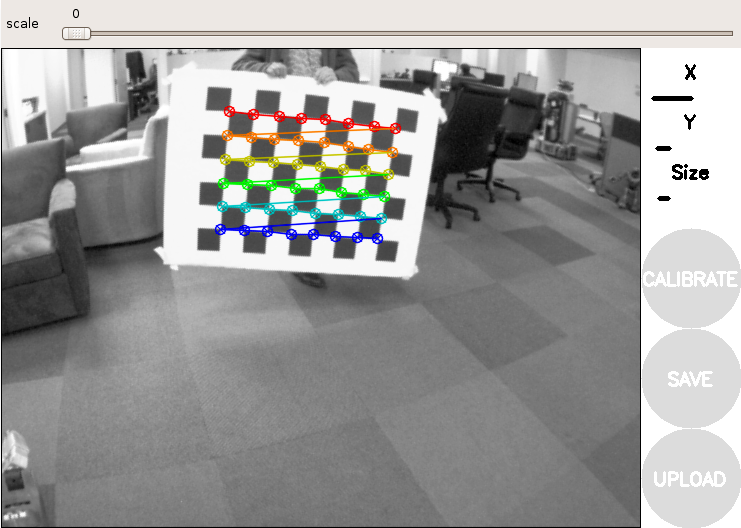
\includegraphics[width=\textwidth]{Img/MonocularCameraCalibration.png}
    \caption{Menú de calibración ROS para cámras monoculares}
    \label{fig:monocularcameracalibration}
\end{figure}

\begin{lstlisting}[caption=Resultado de la calibración en ROS de ejemplo para cámaras monoculares, label=lst:monocularyaml]
image_width: 640
image_height: 480
camera_name: prosilica
camera_matrix:
  rows: 3
  cols: 3
  data: [4827.94,0,1223.5,0,4835.62,1024.5,0,0,1]
distortion_model: plumb_bob
distortion_coefficients:
  rows: 1
  cols: 5
  data: [-0.41527,0.31874,-0.00197,0.00071,0]
rectification_matrix:
  rows: 3
  cols: 3
  data: [1,0,0,0,1,0,0,0,1]
projection_matrix:
  rows: 3
  cols: 4
  data: [4827.94,0,1223.5,0,0,4835.62,1024.5,0,0, 0,1,0]
\end{lstlisting}

\subsubsection{Cámara estéreo}
\textbf{REVISAR TODO ESTO}
Con el fin de poder simular el efecto de la percepción humana, las cámaras estéreo se ubican separadas una distancia fija y, por lo general, alineadas horizontalmente, como se observa en la Figura \ref{fig:stereocamerarig}. Al tener dos fuentes de imágenes distintas y ubicadas en una posición relativa conocida, es posible a partir de las mismas determinar la profundidad en la que se encuentran los objetos que ven entre ambas. 
\begin{figure}[!ht]
    \centering
    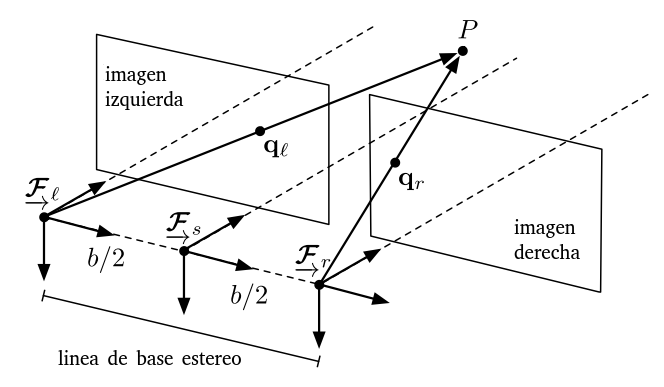
\includegraphics[width=\textwidth]{Img/StereoCameraRig.png}
    \caption{Equipo de cámara estéreo observando un objeto}
    \label{fig:stereocamerarig}
\end{figure}

Si bien esto es posible realizarlo con una cámara monocular, el mismo cuenta de una mayor complejidad y con ciertas restricciones\footnote{Por ejemplo, sería necesario conocer una cierta cantidad de puntos claves del objeto para que, estando el mismo en una pose distinta a la analizada a priori, sea posible determinar la pose del objeto mediante estos puntos claves.}, aunque puede solventarse mediante el agregado de sensores que utilicen otro principio de medición\footnote{Las cámaras RGB-D, por ejemplo, cuentan con una cámara y sensores de distancia para determinar la ubicación de determinados píxeles.}.

Para poder conseguir una imagen estéreo mediante el uso de dos cámaras, deben seguirse una serie de pasos\textbf{(Asano, 2012)}
\begin{enumerate}
    \item Remover las distorsiones de la lente, proceso conocido como \textit{undistortion}\textbf{(QUE PONGO POR UNDISTORTION?)}, explicado anteriormente.
    \item Ajustar las distancias y ángulos entre las cámaras, conocido como \textit{rectificación}.
    \item Encontrar las mismas características en ambas cámaras, proceso conocido como \textit{correspondencia}. A partir de este se consigue un \textit{mapa de disparidad} (o \textit{disparity map}), donde las disparidades son las diferencias en la coordenada x de los planos de la imagen de la misma característica vista en las cámaras izquierda y dercha.
    \item Si se conoce el arreglo geométrico de las cámaras, puede cambiarse el mapa de disparidad en distancias por \textit{triangulación}. Este paso es denominado \textit{proyección}, y el resultado es un mapa de profundidad.
\end{enumerate}

Para obtener buenos resultados, es necesario que las cámaras estén sincronizadas, caso contrario los objetos en movimiento serán un problema.

\paragraph{Matrices características}
Para conocer el arreglo de las cámaras, se utilizan dos matrices características en cámaras estéreo: la \textit{matriz escencial} $E$ y la \textit{matriz fundamental} $F$. La matriz esencial es puramente geométrica, relacionando la ubicación en coordenadas físicas, esto es, rotación y traslación, como se ve en la Figura \ref{fig:essentialgeometry}, del punto $P$ como visto por la cámara izquierda a la ubicación del mismo punto visto por la cámara derecha. En cambio, la matriz fundamental tiene los mismos datos que la matriz esencial, además de relacionar los puntos en el plano de la imagen de una de las cámaras en la otra en coordenadas de imagen.
\begin{figure}
    \centering
    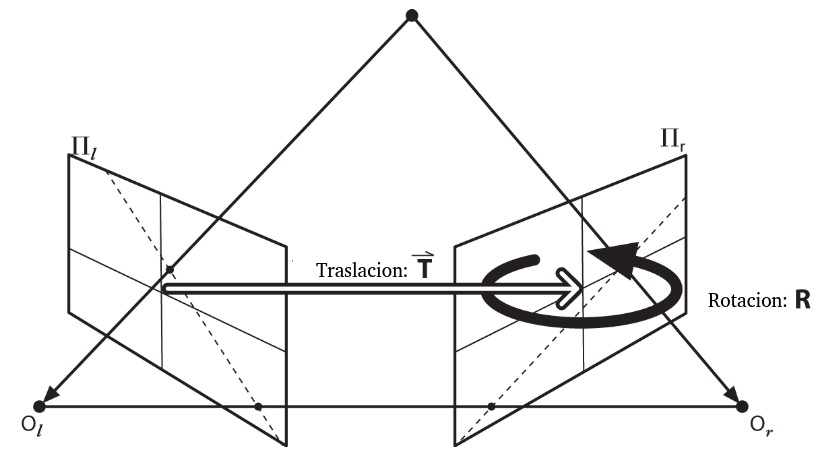
\includegraphics[width=\textwidth]{Img/EssentialGeometry.png}
    \caption{Geometría esencial de la imagen estéreo, recolectada por la matriz esencial $E$}
    \label{fig:essentialgeometry}
\end{figure}

\paragraph{Calibración}
La calibración estéreo depende de hallar la matriz de rotación y la traslación entre las dos cámaras, lo que puede realizarse mediante la función de OpenCV \texttt{cv::stereoCalibrate()}, similar a la función \texttt{cv::cameraCalibrate()} vista anteriormente. En el mismo, se busca una sola matriz de rotación y un vector de traslación que relacione la cámara derecha con la cámara izquierda
\subparagraph{Calibración estéreo mediante ROS}
Para la calibración en ROS puede utilizarse al igual que en cámaras monoculares el paquete \texttt{camera\_calibration}, el cual en este caso recibirá parámetros distintos. La interfaz gráfica para la calibración será similar al de cámaras monoculares, con la diferencia que en este caso aparecen ambas cámaras, aunque el principio de calibración del lado usuario es prácticamente la misma, teniendo en cuenta que ahora en ambas cámaras debe verse el patrón buscado, tal como se observa en la Figura \ref{fig:stereocalibrationchessboard}.
\begin{figure}
    \centering
    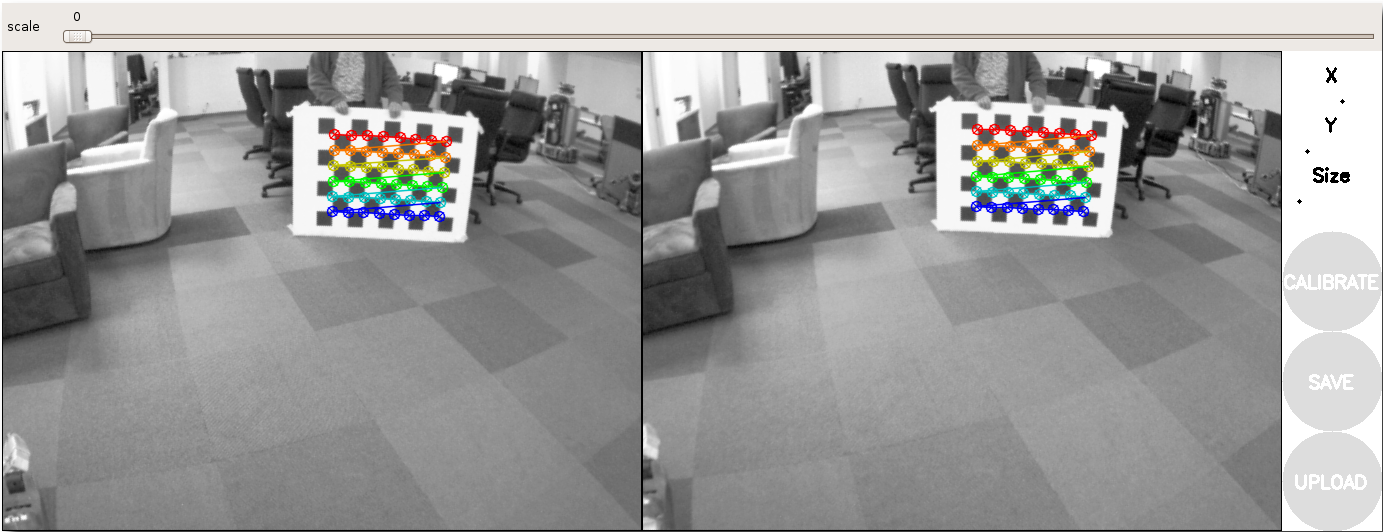
\includegraphics[width=\textwidth]{Img/StereoCalibrationChessboard.png}
    \caption{Calibración estéreo mediante ROS}
    \label{fig:stereocalibrationchessboard}
\end{figure}

En este caso, se obtienen dos archivos YAML, uno para cada cámara, como en el caso de la cámara monocular, aunque las matrices de rectificación y de proyección cobran importancia. La matriz de rectificación es una matriz de rotación que alinea el sistema de coordenadas de la cámara con el plano de imagen estéreo ideal para que las líneas epipolares \textbf{(HABLAR DE EPILOLARES)} en ambas imágenes estéreo sean paralelas. La matriz de proyección

\paragraph{Rectificación estéreo}
Si los planos de ambas cámaras no se encuentran perfectamente alineados, la disparidad estéreo aumenta su complejidad. Para poder mitigar este problema, lo que se busca es reproyectar los planos de la imagen de ambas camaras para que residan en el mismo plano, conocido como \textit{rectificación estéreo}. Dentro de OpenCV, existen numerosas formas de obtenerlo, como pueden ser los algoritmos de Hartley o de Bouguet. El algoritmo de Hartley permite evitar la calibración de la cámara, en cambio para el segundo es necesaria.

Una vez que se obtengan los términos de la calibración estéreo, se pueden calcular previamente los mapas de rectificación izquierda y derecha por separado utilizando para cada uno \texttt{cv::initUndistortRectifyMap()}. El proceso de rectificación estéreo que realiza dicha función puede observarse en la Figura \ref{fig:stereorectification}. Estos pueden luego ser aplicados a cada una de las imágenes mediante un \texttt{cv::remap()}.
\begin{figure}
    \centering
    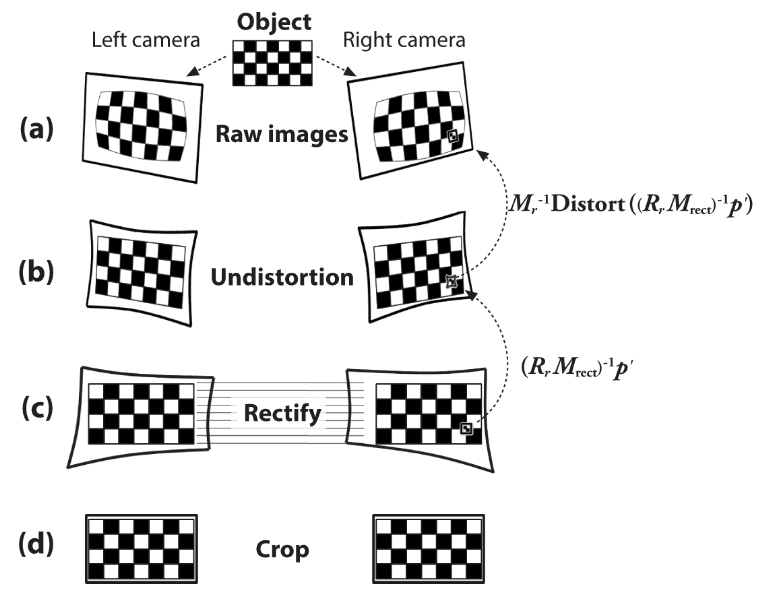
\includegraphics[width=\textwidth]{Img/StereoRectification.png}
    \caption{Rectificación estéreo: Para las cámaras izquierda y derecha, la imagen original (a) se undistorted\textbf{(CHINGAWHAT?!?)} (b) y rectifica (c) y finalmente recortada (d) para enfocarse en áreas superpuestas entre las dos cámaras; el cálculo de rectificación funciona en realidad al revés, o sea, de (c) a (a).}
    \label{fig:stereorectification}
\end{figure}

\subparagraph{Rectificación mediante ROS}
En ROS, el paquete utilizado para dicha tarea es el denominado \texttt{stereo\_image\_proc}\footnote{\url{http://wiki.ros.org/stereo_image_proc}}, que permite obtener un mapa de profundidades.

\paragraph{Correspondencia estéreo}
La correspondencia estéreo, esto es, coincidir un punto tridimensional en las vistas de ambas cámaras, requiere que estos puntos de ambas cámaras se solapen. Para ello, OpenCV implementa dos algoritmos distintos para correspondencias, convirtiendo dos imágenes (izquierda y derecha) en una sola imagen de profundidad
\begin{itemize}
    \item \textit{Block matching (BM) algorithm}, implementada mediante \texttt{cv::StereoBM()}, el cual es rápido y efectivo, aunque en escenas de baja textura presenta problemas. 
    \item \textit{Semi-global block matching (SGBM)}, implementada mediante \texttt{cv::StereoSGBM()}, el cual presenta una mayor exactitud que el BM, pero es computacionalmente más demandante.
\end{itemize}
\subparagraph{Correspondencia utilizando ROS}
Para el caso de ROS, dentro del paquete \texttt{stereo\_image\_proc} se encuentra el ejecutable \texttt{dynamic\_reconfigure}\footnote{\url{http://wiki.ros.org/stereo_image_proc/Tutorials/ChoosingGoodStereoParameters}}, el que permite modificar dinámicamente los parámetros de correspondencia, además de elegir el algoritmo a utilizar mediante una interfaz gráfica.

\subsection{Sensores Inerciales}
El término sensor inercial se usa para denotar la combinación de un acelerómetro de tres ejes y un giroscopio de tres ejes. Los dispositivos que contienen estos sensores se denominan comúnmente unidades de medición inercial (IMU, por \textit{intertial measurement unit}), los cuales en muchos casos incluyen también un magnetómetro de tres ejes. Estas unidades sensoriales suelen ser usadas para determinar la orientación y posición de objetos a los cuales se encuentran integrados, permitiendo así la incorporación de los mismos en gran número de aplicaciones [7, 59, 109, 156] [DE KOK2017].

Hoy en día, muchos de estos sensores se basan en la tecnología de sistemas microelectromecánicos (MEMS). Los componentes de MEMS son pequeños, ligeros, económicos, tienen un bajo consumo de energía y tiempos de arranque cortos. Su precisión ha aumentado significativamente con los años.

Un giroscopio mide la velocidad angular del sensor, es decir, la velocidad de cambio de la orientación del sensor. En cambio, un acelerómetro mide la fuerza específica externa que actúa sobre el sensor. La fuerza específica consiste tanto en la aceleración del sensor como en la gravedad de la Tierra. Por otro lado, los magnetómetros son los encargados de medir el campo magnético en el que el objeto se encuentra sumergido, obteniendo así información absoluta del ambiente y no referida únicamente al objeto en si. Todos estos sensores tienen el inconveniente de presentar un \textit{bias} variable en el tiempo que afecta su funcionamiento, errores de \textit{scaling} utilizados para convertir las salidas digitales de los sensores en cantidades físicas reales, desalineaciones entre ellos mismos en caso de que se trate de un circuito integrado incluyendo a dos o más de ellos, entre otros.

\subsubsection{Calibración}
En una IMU ideal, los grupos triaxiales deben compartir los mismos ejes de sensibilidad ortogonal 3D que abarcan un espacio tridimensional, mientras que el factor de escala debe convertir la cantidad digital medida por cada sensor en la cantidad física real. Desafortunadamente, las IMU basadas en MEMS de bajo costo generalmente se ven afectadas por el escalado no preciso, las desalineaciones del eje del sensor, las sensibilidades de los ejes cruzados y los sesgos distintos de cero. La calibración de la IMU se refiere al proceso de identificación de estas cantidades.

Sin embargo, las IMUs comerciales de costo elevado presentan también estos problemas (aunque en menor escala), con la diferencia de que el fabricante brinda los datos de la calibración, el cual es único para cada una de ellas, minimizando así los términos de incertidumbre. El factor de calibración de estas IMUs se suele realizar con métodos estándar, comparando los datos arrojados por la IMU con referencias conocidas, haciendo que el proceso sea lento y costoso debido al equipamiento necesario. A continuación se presentarán propuestas para resolver la calibración de los diferentes sensores

\paragraph{Acelerómetro-Giróscopo}
Para evitar el uso de equipamiento específico, en \textbf{[TEDALDI2014]} se propone utilizar solo el movimiento propio de la IMU y sus estados intermedios estáticos para calibrar tanto el giróscopo como el acelerómetro. Este procedimiento explota la idea básica del método de múltiples posiciones, presentado primero en [7] para la calibración de acelerómetros: en una posición estática, las normas de las aceleraciones medidas son iguales a las magnitudes de la gravedad más un multi-factor de error de origen (es decir, incluye \textit{bias}, desalineación, ruido, entre otros). Todas estas cantidades pueden estimarse a través de la minimización sobre un conjunto de actitudes estáticas. 

Después de la calibración de la tríada del acelerómetro, es posible utilizar las posiciones del vector de gravedad medidas por los acelerómetros como referencia para calibrar la tríada del giroscopio. Es por esto que la exactitud de la calibración del giroscopo depende fuertemente de la exactitud de la calibración del acelerómetro. Al integrar las velocidades angulares entre dos posiciones estáticas consecutivas, se consigue estimar las posiciones de gravedad en la nueva orientación. La calibración de los giroscopios finalmente se obtiene minimizando los errores entre estas estimaciones y las referencias de gravedad dadas por los acelerómetros calibrados.

Para una IMU ideal, los 3 ejes de la tríada de acelerómetros y los 3 ejes de la tríada de giroscopios definen un marco tridimensional único, compartido y ortogonal. En la realidad, en base a lo explicado anteriormente, los marcos de los acelerómetros y de los giróscopos no suelen ser ortogonales. A su vez, si se tiene a ambos dentro de un mismo chip, puede definirse un marco del cuerpo (o body frame), el cual es un marco ortogonal que representa, por ejemplo, el chasis del integrado. Este marco suele ser distinto a los otros dos marcos, pero como esta diferencia está dada por ángulos muy pequeños, la medición $\bm{m}$ tanto del acelerómetro como del giróscopo en un marco no ortogonal (o sea, el marco del sensor) puede llevarse al marco del cuerpo mediante
\begin{equation}
    \bm{m}^b = \bm{C}\bm{m}^s
\end{equation}
siendo $\bm{C}$ la matriz de rotación de la Expresión (\ref{eq:rpyinfinitesimal}).

Si se asume que el marco del cuerpo coincide con el marco ortogonal del acelerómetro, entonces para el caso de la aceleración
\begin{equation}
    \bm{a}^b = \bm{C}_a\bm{a}^s
\end{equation}
siendo
\begin{equation}
    \bm{C}_a =
    \begin{bmatrix}
        1 & \alpha_{12} & \alpha_{13} \\
        0 & 1 & \alpha_{23} \\
        0 & 0 & 1
    \end{bmatrix}
\end{equation}
Como se mencionó anteriormente, tanto las mediciones del acelerómetro como las del giróscopo deberían referir al mismo marco de referencia, en este caso, el marco del cuerpo. Por lo tanto,
\begin{equation}
    \bm{\omega}^b = \bm{C}_g\bm{\omega}^s
\end{equation}
siendo
\begin{equation}
    \bm{C}_g =
    \begin{bmatrix}
        1 & \gamma_{12} & \gamma_{13} \\
        \gamma_{21} & 1 & \gamma_{23} \\
        \gamma_{31} & \gamma_{32} & 1
    \end{bmatrix}
\end{equation}

Debido al error en la conversión, ambos sensores se encuentran afectados por errores de \textit{scaling}
\begin{align}
    \bm{K}_a &=
    \begin{bmatrix}
        sa_x & 0 & 0 \\
        0 & sa_y & 0 \\
        0 & 0 & sa_z
    \end{bmatrix}
    \\
    \bm{K}_g &=
    \begin{bmatrix}
        sg_x & 0 & 0 \\
        0 & sg_y & 0 \\
        0 & 0 & sg_z
    \end{bmatrix}
\end{align}
 y de \textit{bias}
 \begin{align}
    \bm{b}_a &=
    \begin{bmatrix}
        ba_x \\
        ba_y \\
        ba_z
    \end{bmatrix}
    \\
     \bm{b}_a &=
     \begin{bmatrix}
        bg_x \\
        bg_y \\
        bg_z
     \end{bmatrix}
\end{align}

En consecuente, los modelos completos de los sensores resultan
\begin{align}
    \bm{a}^b &= \bm{C}_a\bm{K}_a\left(\bm{a}^s + \bm{b}_a + \bm{v}_a\right) \\
    \bm{\omega}^b &= \bm{C}_g\bm{K}_g\left(\bm{\omega}^s + \bm{b}_g + \bm{v}_g\right)
\end{align}
con $\bm{v}_i$ correspondiendo a los ruidos de medición de cada uno.

En concreto, para cada uno de los sensores se tendrán parámetros a estimar. Para el caso del acelerómetro
\begin{equation}
    \bm{\epsilon}_{a} = [\alpha_{12},\alpha_{13},\alpha_{23},sa_x,sa_y,sa_z,ba_x,ba_y,ba_z]
    \label{eq:accelcalibrationparams}
\end{equation}

Al aplicarse un promediado a cada intervalo de la calibración del acelerómetro, esto permite olvidar el ruido de la medición, y definir entonces
\begin{equation}
    \bm{a}^b = h(\bm{a}^s,\bm{\epsilon}_{a}) = \bm{T}_a\bm{K}_a(\bm{a}^s+\bm{b}_a)    
\end{equation}

Como en [7], se mueve a la IMU un set de $M$ rotaciones independientes y temporalmente estables, obteniendo entonces $M$ aceleraciones $\bm{a}^s_k$, las cuales son promediadas en cada uno de estos intervalos estáticos. La función de coste para minimizar los parámetros este caso es
\begin{equation}
    \mathscr{S}(\bm{\epsilon}_{a}) = \sum_{k=1}^M(||\bm{g}||^2-||h(\bm{a}^s_k,\bm{\epsilon}_{a})||^2)^2
    \label{eq:generalaccelcostfunction}
\end{equation}
donde $||g||^2$ es la magnitud actual del vector de gravedad local, obtenido de tablas específicas.

Para calibrar la triada del giróscopo, puede asumirse al mismo libre de \textit{bias} ya que este sesgo puede obtenerse promediando sobre una cantidad de datos consecutivos de tamaño conveniente en el instante inicial estacionario. Por ello, el vector de parámetro desconocidos resulta
\begin{equation}
    \bm{\epsilon}_{g} = \left[\gamma_{12},\ \gamma_{13},\ \gamma_{21},\ \gamma_{23},\ \gamma_{31},\ \gamma_{32},\ sg_x,\ sg_y,\ sg_z\right]
    \label{eq:gyrocalibrationparams}
\end{equation}

Una vez definido el \textit{bias}, como para la calibración del giróscopo se toma al acelerómetro como referencia conocida, se requiere convertir los datos de dicho giróscopo en un vector de aceleraciones. Para ello, se define el operador $\psi$, 
\begin{equation}
    \bm{u}_{g,k} = \psi\left[\bm{\omega}_i^s,\bm{u}_{a,k-1}\right]
\end{equation}
que toma como entrada una secuencia de $n$ lecturas del giróscopo $\bm{\omega}_i^s$ y el versor de gravedad inicial $\bm{u}_{a,k-1}$ obtenido del acelerómetro ya calibrado, y retorna el versor de gravidad final $\bm{u}_{g,k}$. 
Una vez obtenido $\bm{u}_{g,k}$, para el caso del giróscopo, la función de coste será entonces
\begin{equation}
    \mathscr{S}(\bm{\epsilon}_{g}) = \sum_{k=2}^M ||\bm{u}_{a,k} - \bm{u}_{g,k}||^2
\end{equation}
siendo $M$ el número de los intervalos estáticos, $\bm{u}_{a,k}$ es el versor de la aceleración medido promediando en la ventana temporal obtenida en el $k$-ésimo intervalo estático, y $\bm{u}_{g,k}$ corresponde al versor de aceleración en base a los datos del giróscopo computada anteriormente. Se obtiene, entonces, $\bm{\epsilon}_{g}$ minimizando la Expresión anterior..

\subparagraph{Ecuación diferencial ordinaria de la velocidad angular}
Si se tiene un vector $\bm{r}$ de longitud constante, la velocidad angular del mismo en base a las leyes físicas puede obtenerse realizando la derivada del mismo
\begin{equation}
    \frac{d\bm{r}}{dt} = \bm{\omega}\times \bm{r}
\end{equation}
siendo $\times$ el producto externo. Como para el caso evaluado la velocidad angular es perpendicular al vector $\bm{r}$ (producto intero $\bm{\omega}\cdot\bm{r} = 0$), tal como puede verse en la Figura \ref{fig:angularvelocity}. Por lo tanto, puede escribirse a la misma en la forma de cuaterniones
\begin{equation}
    \frac{d\bm{r}}{dt} = \bm{\omega} \otimes \bm{r}
\end{equation}
teniendo en cuenta que tanto $\bm{\omega}$ como $\bm{r}$ se obtienen mediante la Expresión (\ref{eq:vectorquaternionform}).

\textbf{REVISAR SI ESTA BIEN EL GRAFICO, LA IDEA !!!}
\begin{figure}[!ht]
    \centering
    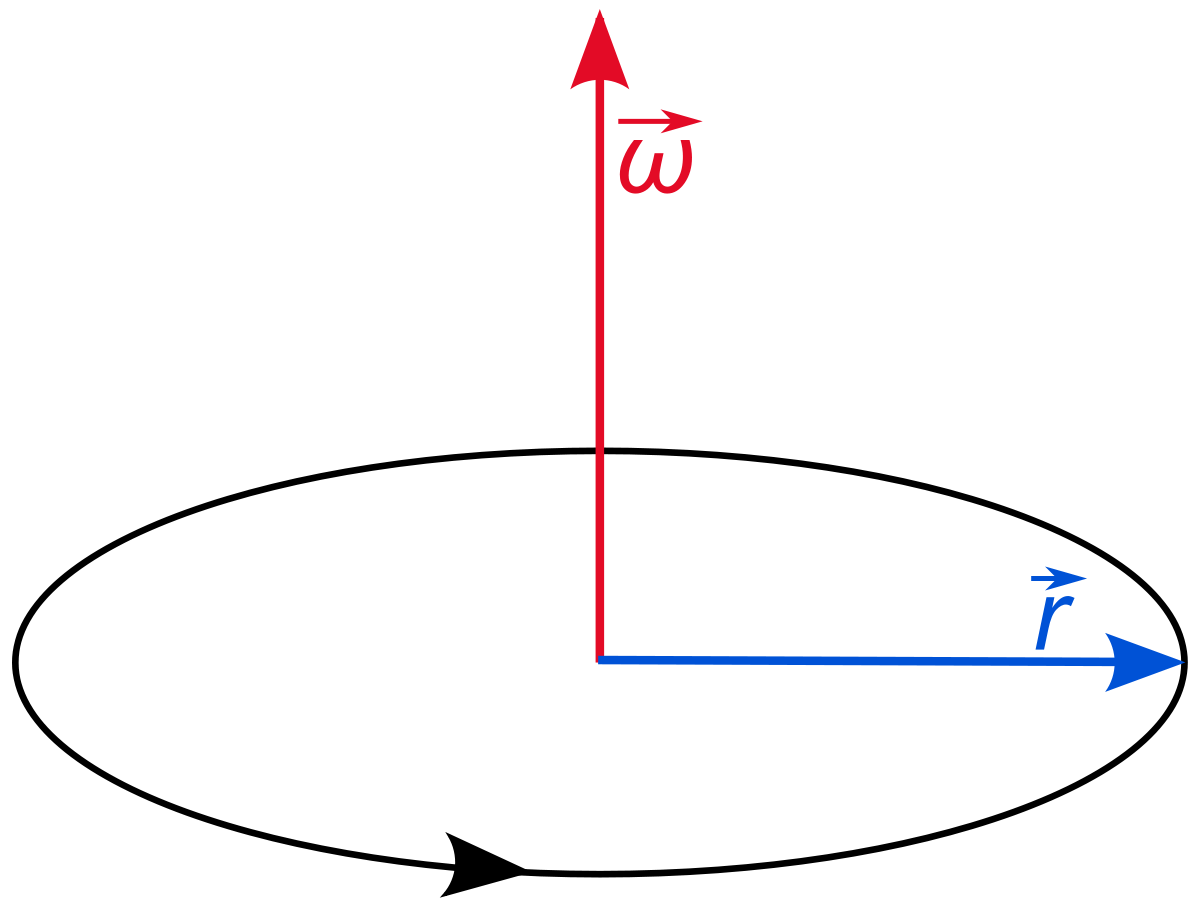
\includegraphics[width=0.5\textwidth]{Img/AngularVelocity.png}
    \caption{Velocidad angular respecto al vector}
    \label{fig:angularvelocity}
\end{figure}

Ahora, siendo que $\bm{r}$ puede definirse mediante la Expresión (\ref{eq:quaternionvectorrotation}), y teniendo en cuenta las propiedades de los cuaterniones
\begin{align}
    \bm{r} &= \bm{q}\otimes \bm{r}_0 \otimes \bm{q}^{-1} \\
    \frac{d\bm{r}}{dt} &= \frac{d}{dt}\left[\bm{q}\otimes\bm{r}_0\otimes\bm{q}^{-1}\right] \\
    &= \dot{\bm{q}}\otimes\bm{r}_0\otimes\bm{q}^{-1} + \bm{q}\otimes\bm{r}_0\otimes\dot{\bm{q}^{-1}} = \bm{\omega}\otimes\bm{r}
\end{align}

Como $\dot{\bm{q}^{-1}}$ puede generar problemas, es posible obtenerlo realizando la derivada del conjugado del cuaternión con su conjugado
\begin{align}
    \frac{d}{dt}\left(\bm{q}\otimes\bm{q}^{-1}\right) &= \frac{d}{dt}1 \\
    \dot{\bm{q}}\otimes\bm{q}^{-1} + \bm{q}\otimes\dot{\bm{q}^{-1}} &= 0
\end{align}
entonces
\begin{equation}
    \dot{\bm{q}^{-1}} = -\bm{q}^{-1}\otimes\dot{\bm{q}}\otimes\bm{q}^{-1}
\end{equation}
sustituyendo y poniéndolo en función de $\bm{r}$
\begin{equation}
        \frac{d}{dt}\left[\bm{q}\otimes\bm{r}_0\otimes\bm{q}^{-1}\right] = \dot{\bm{q}}\otimes\bm{q}^{-1}\otimes\bm{r} - \bm{r}\otimes\dot{\bm{q}}\otimes\bm{q}^{-1}
\end{equation}
donde dicha Expresión tiene la forma de la operación conmutador $\left[\bm{p},\bm{q}\right]$. Finalmente, puede llegarse a la ecuación diferencial
\begin{align}
    \dot{\bm{q}}\otimes\bm{q}^{-1}\otimes\bm{r} - \bm{r}\otimes\dot{\bm{q}}\otimes\bm{q}^{-1} &= \bm{\omega}\otimes\bm{r} \\
    \left[\dot{\bm{q}}\otimes\bm{q}^{-1},\bm{r}\right] &= \bm{\omega}\otimes\bm{r} \\
    2\dot{\bm{q}}\otimes\bm{q}^{-1}\otimes\bm{r} &= \bm{\omega}\otimes\bm{r} \\
    \dot{\bm{q}} &= \frac{1}{2}\bm{\omega}\otimes\bm{q}
    \label{eq:quaternionedoglobalframe}
\end{align}
donde $\bm{\omega}(t)$ es la velocidad angular en el marco fijo global\textbf{(Sola, 2017)}. En muchos casos es útil formular la Expresión (\ref{eq:quaternionedoglobalframe}) en base a la velocidad angular en el marco del sensor. La velocidad angular en este marco es la velocidad angular global rotada en el marco del cuerpo, dado por la Expresión (\ref{eq:quaternionvectorrotation}). En consecuencia,
\begin{equation}
    \dot{\bm{q}} = \frac{1}{2}\bm{q}\otimes\bm{\omega}^s\otimes\bm{q}^{-1}\otimes\bm{q}
\end{equation}
y recordando la Propiedad (\ref{eq:quaternioninverse})
\begin{equation}
    \dot{\bm{q}} = \frac{1}{2}\bm{q}\otimes\bm{\omega}^s 
\end{equation}
Finalmente, en base a la Expresión (\ref{eq:quaternionproductmatrixright}), se llega a
\begin{equation}
    \dot{\bm{q}} = \frac{1}{2}\bm{\Omega}(\bm{\omega}(t))\bm{q}
    \label{eq:edoquaternion}
\end{equation}
siendo $\bm{\Omega}(\bm{\omega}(t))$ la matriz de rotación en base a la velocidad angular obtenida del giróscopo
\begin{equation}
    \bm{\Omega}(\bm{\omega}(t)) =
    \begin{bmatrix}
        0 & -\bm{\omega} \\
        \bm{\omega}^T & -\left[\bm{\omega}\right]_\times
    \end{bmatrix}
    =
    \begin{bmatrix}
        0 & -\omega_x & -\omega_y & -\omega_z \\
        \omega_x & 0 & \omega_z & -\omega_y \\
        \omega_y & -\omega_z & 0 & \omega_x \\
        \omega_z & \omega_y & -\omega_x & 0
    \end{bmatrix}
\end{equation}

\paragraph{Magnetómetro}
Para la calibración del magnetómetro, en cambio, los enfoques tradicionales suponen que hay un sensor de referencia disponible que puede proporcionar información de rumbo precisa. Un ejemplo bien conocido de esto es el balanceo de la brújula [3]. Sin embargo, para permitir que cualquier usuario realice la calibración, se han desarrollado una gran cantidad de enfoques que eliminan la necesidad de una fuente de información de orientación. Una clase de estos algoritmos de calibración de magnetómetro se enfoca en minimizar la diferencia entre la magnitud del campo magnético medido y la del campo magnético local[4]. Este enfoque también se conoce como verificación escalar[5]. Otra clase formula el problema de calibración como un problema de ajuste de elipsoide, es decir, como el problema de mapear un elipsoide de datos a una esfera[6] - [8]. El beneficio de usar esta formulación es que existe una vasta literatura sobre cómo resolver problemas de ajuste de elipsoides,[9][10]. Fuera de estas dos clases, también está disponible un gran número de otros enfoques de calibración[11], donde se consideran diferentes formulaciones del problema de calibración en términos de un problema de máxima verosimilitud. La ventaja de estos métodos es que utilizan sólo la información provista por el magnetómetro.

Sin embargo, si lo que se busca es calibrar un magnetómetro para mejorar la estimación del rumbo en combinación con sensores inerciales, la alineación de los ejes sensoriales de los sensores de inercia y el magnetómetro es crucial en este caso. Se puede ver que esta alineación determina la orientación de la esfera azul de los datos del magnetómetro calibrado en la Fig. 1. Los algoritmos que solo usan datos del magnetómetro pueden asignar el elipsoide rojo de los datos a una esfera, pero sin información adicional, la rotación de esta esfera permanece desconocido.

Varios enfoques más modernos incluyen un segundo paso en el algoritmo de calibración para determinar la desalineación[6], [12] - [14] entre diferentes ejes del sensor. Una opción común para alinear los ejes del sensor de inercia y el magnetómetro es utilizar mediciones de acelerómetro a partir de períodos de aceleraciones bastante pequeñas [12], [13]. La desventaja de este enfoque es que se debe determinar un umbral para usar las mediciones del acelerómetro. Además, se omiten los datos del giroscopio. En [15], por otro lado, el problema se reformula en términos del cambio de orientación, lo que permite el uso directo de los datos del giroscopio. \textbf{[DE KOK 2014]}


\subsection{Encoders}
El objetivo de los encoders es medir las rotaciones relativas de la rueda a la que están asociados. Los encoders normalmente se fijan a la salida del motor o de la caja de cambios, con opciones de diseño que a menudo cambian la resolución angular con la máxima velocidad. Los efectos de resolución y muestreo a menudo producen mediciones ruidosas que requieren filtrado digital. La odometría basada en ruedas supone que no hay deslizamiento entre las ruedas y el terreno. En la práctica, los robots móviles con frecuencia superan la fricción estática y rodante, y cuando una o más ruedas giran o se deslizan, pueden ocurrir grandes errores de odometría. La pendiente del terreno, la fricción y otras propiedades pueden variar, incluso entre ruedas individuales. Los robots de accionamiento diferencial con cuatro ruedas a menudo experimentan grandes errores de odometría cuando giran, ya que se requiere un deslizamiento de las ruedas para girar [150].

\subsection{GPS}
El GPS es un sistema de navegación georreferenciado basado en satélites mediante los cuales estima la latitud, longitud y altitud del objeto en cuestión. Debido a esto, el mismo tiene su campo de aplicación principalmente en ambientes al aire libre, donde mediante la triangulación entre 4 o más satélites puede determinar la ubicación del objeto en cuestión. Debido a esto y a que, entre otros factores, su principio de funcionamiento se basa en medir el tiempo que tardó la señal disparada por un satélite en ser recibida por el propio sensor, el mismo cuenta con precisiones variables dependiendo de la posición de los satélites [162]. Estos sesgos y errores de grandes pasos hacen que la navegación robótica con GPS sea problemática, especialmente con grandes equipos de robots que operan en entornos urbanos y durante muchas horas. [CARLSON2010]